
\documentclass[14pt]{beamer}
\usepackage{listings}


\input{/home/frr/SYNC/Dropbox/Modelos/Modelo_apresentacao_beamer/conf_slides}

\title[]{\huge Tópicos Especiais I - Desenvolvimento aplicações móveis}
\subtitle{Apresentação}


\institute[Apresentação]{}
\author[]{
\includegraphics[width=1.8cm]{/home/frr/SYNC/Dropbox/Modelos/Modelo_apresentacao_beamer/logo}\\Prof. Dr. Fábio Rodrigues de la Rocha}
\date[]{}
%\pgfdeclareimage[width=1.2cm]{logo}{imagens/logo}


\begin{document}


\frame{\titlepage}


%%%%%%%%%%%%%%%%%%%%%%%%%%%%%%%%%%%%%%%%%%%%%%%%%%%%%%%%%%%5

\begin{frame}\frametitle{Sumário}
\begin{itemize}
\item Sobre o que trata a disciplina ?
\pause
\item Página da disciplina http://fabiodelarocha.paginas.ufsc.br/
\pause
\item Aulas, provas, trabalhos
\pause 
\item Linux, Ambiente de programação, Programação em NodeJS, Programação híbrida para smartfones (Android)
\pause
\item Plano de ensino

\end{itemize}
\end{frame}

%%%%%%%%%%%%%%%%%%%%%%%%%%%%%%%%%%%%%%%%%%%%%%%%%%%%%%%%%%%5

\begin{frame}\frametitle{Introdução}

\begin{block}{Clientes e servidores WEB}

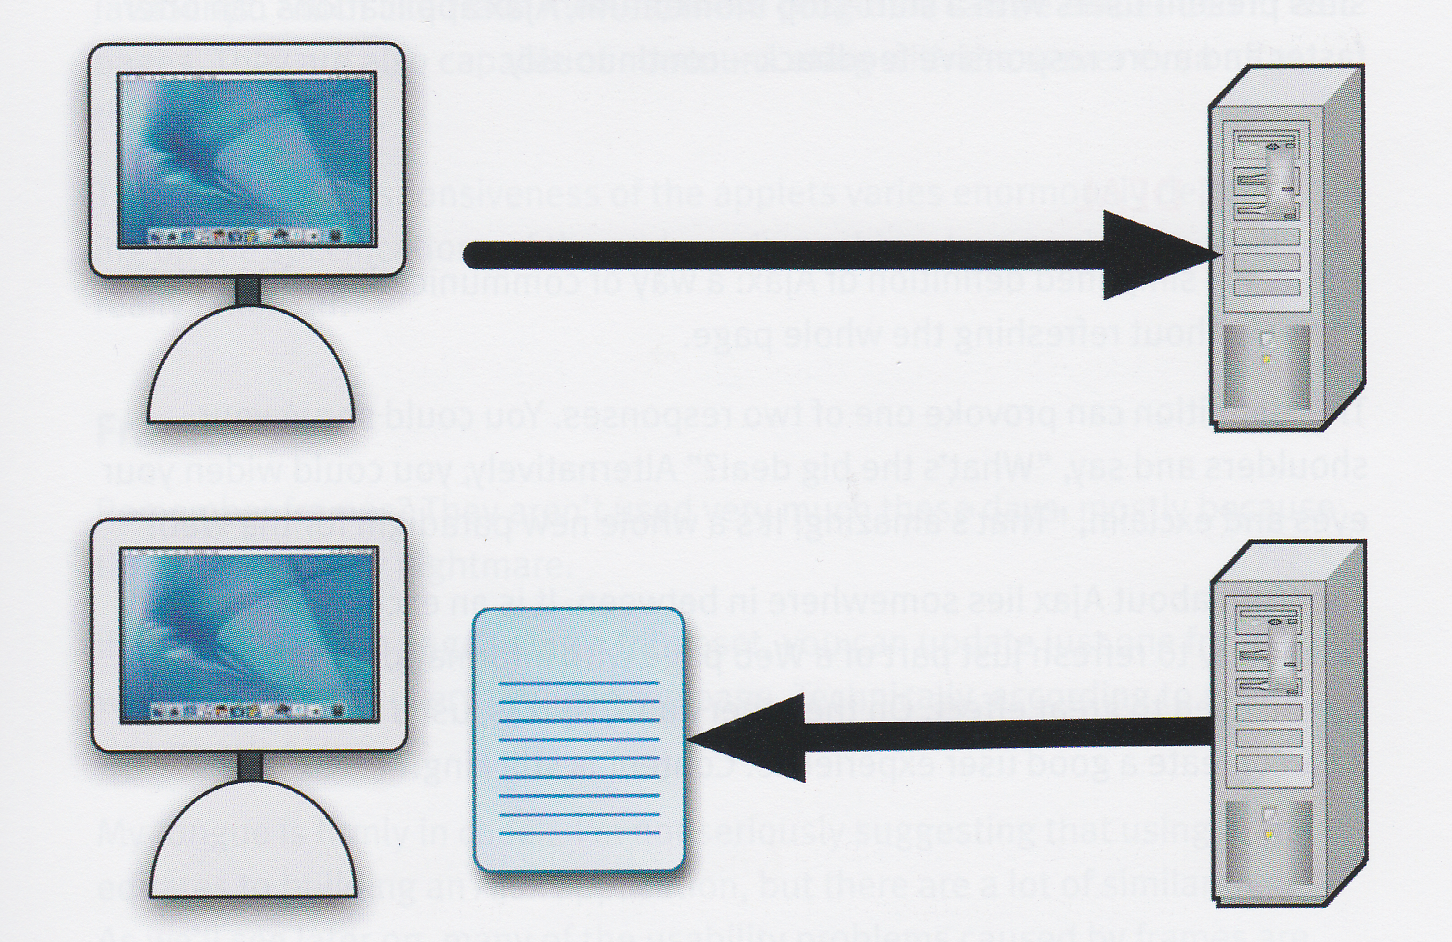
\includegraphics[width=0.8\textwidth]{clienteServidor}

\end{block}

\end{frame}

%%%%%%%%%%%%%%%%%%%%%%%%%%%%%%%%%%%%%%%%%%%%%%%%%%%%%%%%%%
\begin{frame}[fragile]
 \frametitle{Exemplo:Abrindo e fechando arquivos}
\begin{lstlisting}[basicstyle=\tiny\ttfamily]
<html>
  <body>
    <a href="http://www.google.com>GOOGLE</a>
    <a href="http://www.ufsc.br>UFSC</a>
    <img src="http://ararangua.ufsc.br/files/2017/09/cropped-Logo-UFSC.png" alt="figura" />
  
  </body>
</html>
\end{lstlisting}

\end{frame}
%%%%%%%%%%%%%%%%%%%%%%%%%%%%%%%%%%%%%%%%%%%%%%%%%%%%%%%%%%%



%%%%%%%%%%%%%%%%%%%%%%%%%%%%%%%%%%%%%%%%%%%%%%%%%%%%%%%%%%
\begin{frame}[fragile]
 \frametitle{tópicos}
\begin{itemize}
 \item GET, POST
 \item refresh de página
 \item Modelo com JS
\end{itemize}


\end{frame}
%%%%%%%%%%%%%%%%%%%%%%%%%%%%%%%%%%%%%%%%%%%%%%%%%%%%%%%%%%%

%%%%%%%%%%%%%%%%%%%%%%%%%%%%%%%%%%%%%%%%%%%%%%%%%%%%%%%%%%
\begin{frame}[fragile]
 \frametitle{Javascript}
\begin{itemize}
 \item O que é ? para que serve ?
 \item 
 \item AJAX
\end{itemize}


\end{frame}
%%%%%%%%%%%%%%%%%%%%%%%%%%%%%%%%%%%%%%%%%%%%%%%%%%%%%%%%%%%

%%%%%%%%%%%%%%%%%%%%%%%%%%%%%%%%%%%%%%%%%%%%%%%%%%%%%%%%%%
\begin{frame}[fragile]
 \frametitle{Arquivo HTML}
\begin{lstlisting}[basicstyle=\tiny\ttfamily]
<html>
  <script>
  function carrega () {
    var xhttp = new XMLHttpRequest();
    xhttp.onreadystatechange = function() {
      if (this.readyState == 4 && this.status == 200) {
	document.getElementById("demo").innerHTML = xhttp.responseText;
      }
    };
    xhttp.open("GET", "/conteudo", true);
    xhttp.send();
   }
   
  </script>
  
  <body>
    <a href="http://www.google.com">GOOGLE</a>
    <a href="http://www.ufsc.br">UFSC</a>
    <img src="http://ararangua.ufsc.br/files/2017/09/cropped-Logo-UFSC.png" alt="figura" />
      <button  onclick="carrega()" >Carrega</button>
    <div id="demo"  >
      teste teste teste
    </div>
  </body>
</html>
\end{lstlisting}

\end{frame}
%%%%%%%%%%%%%%%%%%%%%%%%%%%%%%%%%%%%%%%%%%%%%%%%%%%%%%%%%%%

\end{document}
